
\documentclass{standalone}
\usepackage{tikz}
\usepackage{../mss}
\usepackage{sansmath}

\usetikzlibrary{shapes.geometric,positioning,calc,petri,graphs,fit,backgrounds}
\tikzset{
node distance=0.5cm and 0.5cm,
>=latex,
font=\sf\bfseries\sansmath,
,
textfeld/.style={align=center,minimum height=0.5cm,minimum width=1.5cm},
pfeil/.style={->,line width=1.1pt},
box/.style={rectangle,draw,line width=1.1pt,minimum height=1.5cm,minimum width=2.8cm,align=center},
place/.style={circle,line width=1.1pt,draw=black,minimum size=6mm},
transition/.style={rectangle,line width=1.1pt,draw=black,minimum size=6mm},
every edge/.append style={line width=1.1pt}
module/.style={rectangle,draw,fill,line width=1.1pt,minimum height=1.5cm,minimum width=2.8cm,align=center},
marking/.style={align=center,inner sep=1pt},
initial/.style={draw=none}
}
\tikzgraphsset{
    every graph/.style = {use existing nodes}
}

\begin{document}


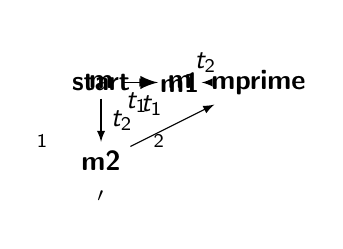
\begin{tikzpicture}
    \node[marking] (m) {$ \marking $};
    \node[below left=of m] (m1) {$ \marking_1 $};
    \node[below right=of m] (m2) {$ \marking_2 $};
    \coordinate(mid) at ($(m1)!0.5!(m2)$) ;

    \node[below =of mid] (mprime) {$ \marking^\prime $};

    \graph{
    m ->[edge label'={$ t_1 $}] m1 ->[edge label'={$ t_2 $}] mprime, m ->[edge label={$ t_2 $}] m2 ->[edge label={$ t_1 $}] mprime
    };

    \node[initial, above left=2.5mm and 1.5mm of m] (start) {};
    \graph{start ->[line width=1.2pt] m};
\end{tikzpicture}

\end{document}